%\documentclass{beamer}
\documentclass[accentcolor=tud9c,colorbacktitle,inverttitle,landscape,german,presentation]{tudbeamer}
\usepackage[english]{babel}
\usepackage[utf8]{inputenc}
\usepackage{amsmath}
\usepackage[justification=centering]{caption}
\usepackage{booktabs}
\providecommand\thispdfpagelabel[1]{} % Hack fuer Inkompatibiltitaet zur Latex-Beamer-Klasse

\begin{document}

\title[]{Workshop on Representation Learning for NLP}
\subtitle{11 August, 2016, Berlin, Germany}

%%%%%%%%%%%%%%%%%%%%%%%%%%%%%%%%%%%%%%%%%%%%%%%%%%%%%%%%%%%%%%%%%%%%%%%%%%%%%%%%%%%%%%%%%%%%%%%%%%%%%%%%%%%%%%%%%%%%%%%%%%%%%%%%%%%%%%%%%%%%
\begin{titleframe}
	\vspace{1cm}	
	\begin{center}
		\LARGE \alert{\textbf{	
			Making Sense of Word Embeddings \\
		}}	
		\vspace{0.7cm}
		\small Maria Pelevina$^1$, Nikolay Arefyev$^2$, Chris Biemann$^1$ and \textbf{Alexander Panchenko}$^1$
		
		\vspace{1.3cm}
		\scriptsize $^1$Technische Universit{\"a}t Darmstadt, LT Group, Computer Science Department, Germany\\
		
		\scriptsize $^2$Moscow State University, Faculty of Computational Mathematics and Cybernetics, Russia
	\end{center}
\end{titleframe}

%%%%%%%%%%%%%%%%%%%%%%%%%%%%%%%%%%%%%%%%%%%%%%%%%%%%%%%%%%%%%%%%%%%%%%%%%%%%%%%%%%%%%%%%%%%%%%%%%%%%%%%%%%%%%%%%%%%%%%%%%%%%%%%%%%%%%%%%%%%%
\begin{frame}{Overview of the contribution}

	\begin{block}{Prior methods:}
		\vspace{0.25cm}

	\begin{itemize}	
	\item Induce inventory by \alert{clustering of word instances} (Li and Jurafsky, 2015)
	\item Use existing inventories (Rothe and Sch\"{u}tze, 2015)	
	\end{itemize}
\end{block}


	\begin{block}{Our method:}
		\vspace{0.25cm}

	\begin{itemize}	
	\item \textbf{Input:} word embeddings
	\item \textbf{Output:} word sense embeddings
	\item \textbf{Word sense induction} by \alert{clustering of word ego-networks}
	\item \textbf{Word sense disambiguation} based on the induced sense representations
	
	\end{itemize}
\end{block}

%	\item A method for unsupervised word sense induction and disambiguation}}	
%	
%	\vspace{0.5cm}
%	
%	\begin{block}{Word Sense Induction:}
%		\vspace{0.25cm}
%		\begin{itemize}
%			\item via clustering of \textbf{word ego-networks}
%		\end{itemize}
%	\end{block}
%	
%	\begin{block}{Word Sense Disambiguation:}
%		\begin{itemize}
%			\item using \textbf{vector representations} of context words and word senses
%		\end{itemize}
%	\end{block}
\end{frame}

%%%%%%%%%%%%%%%%%%%%%%%%%%%%%%%%%%%%%%%%%%%%%%%%%%%%%%%%%%%%%%%%%%%%%%%%%%%%%%%%%%%%%%%%%%%%%%%%%%%%%%%%%%%%%%%%%%%%%%%%%%%%%%%%%%%%%%%%%%%%


\begin{frame}{Learning Word Sense Embeddings}
	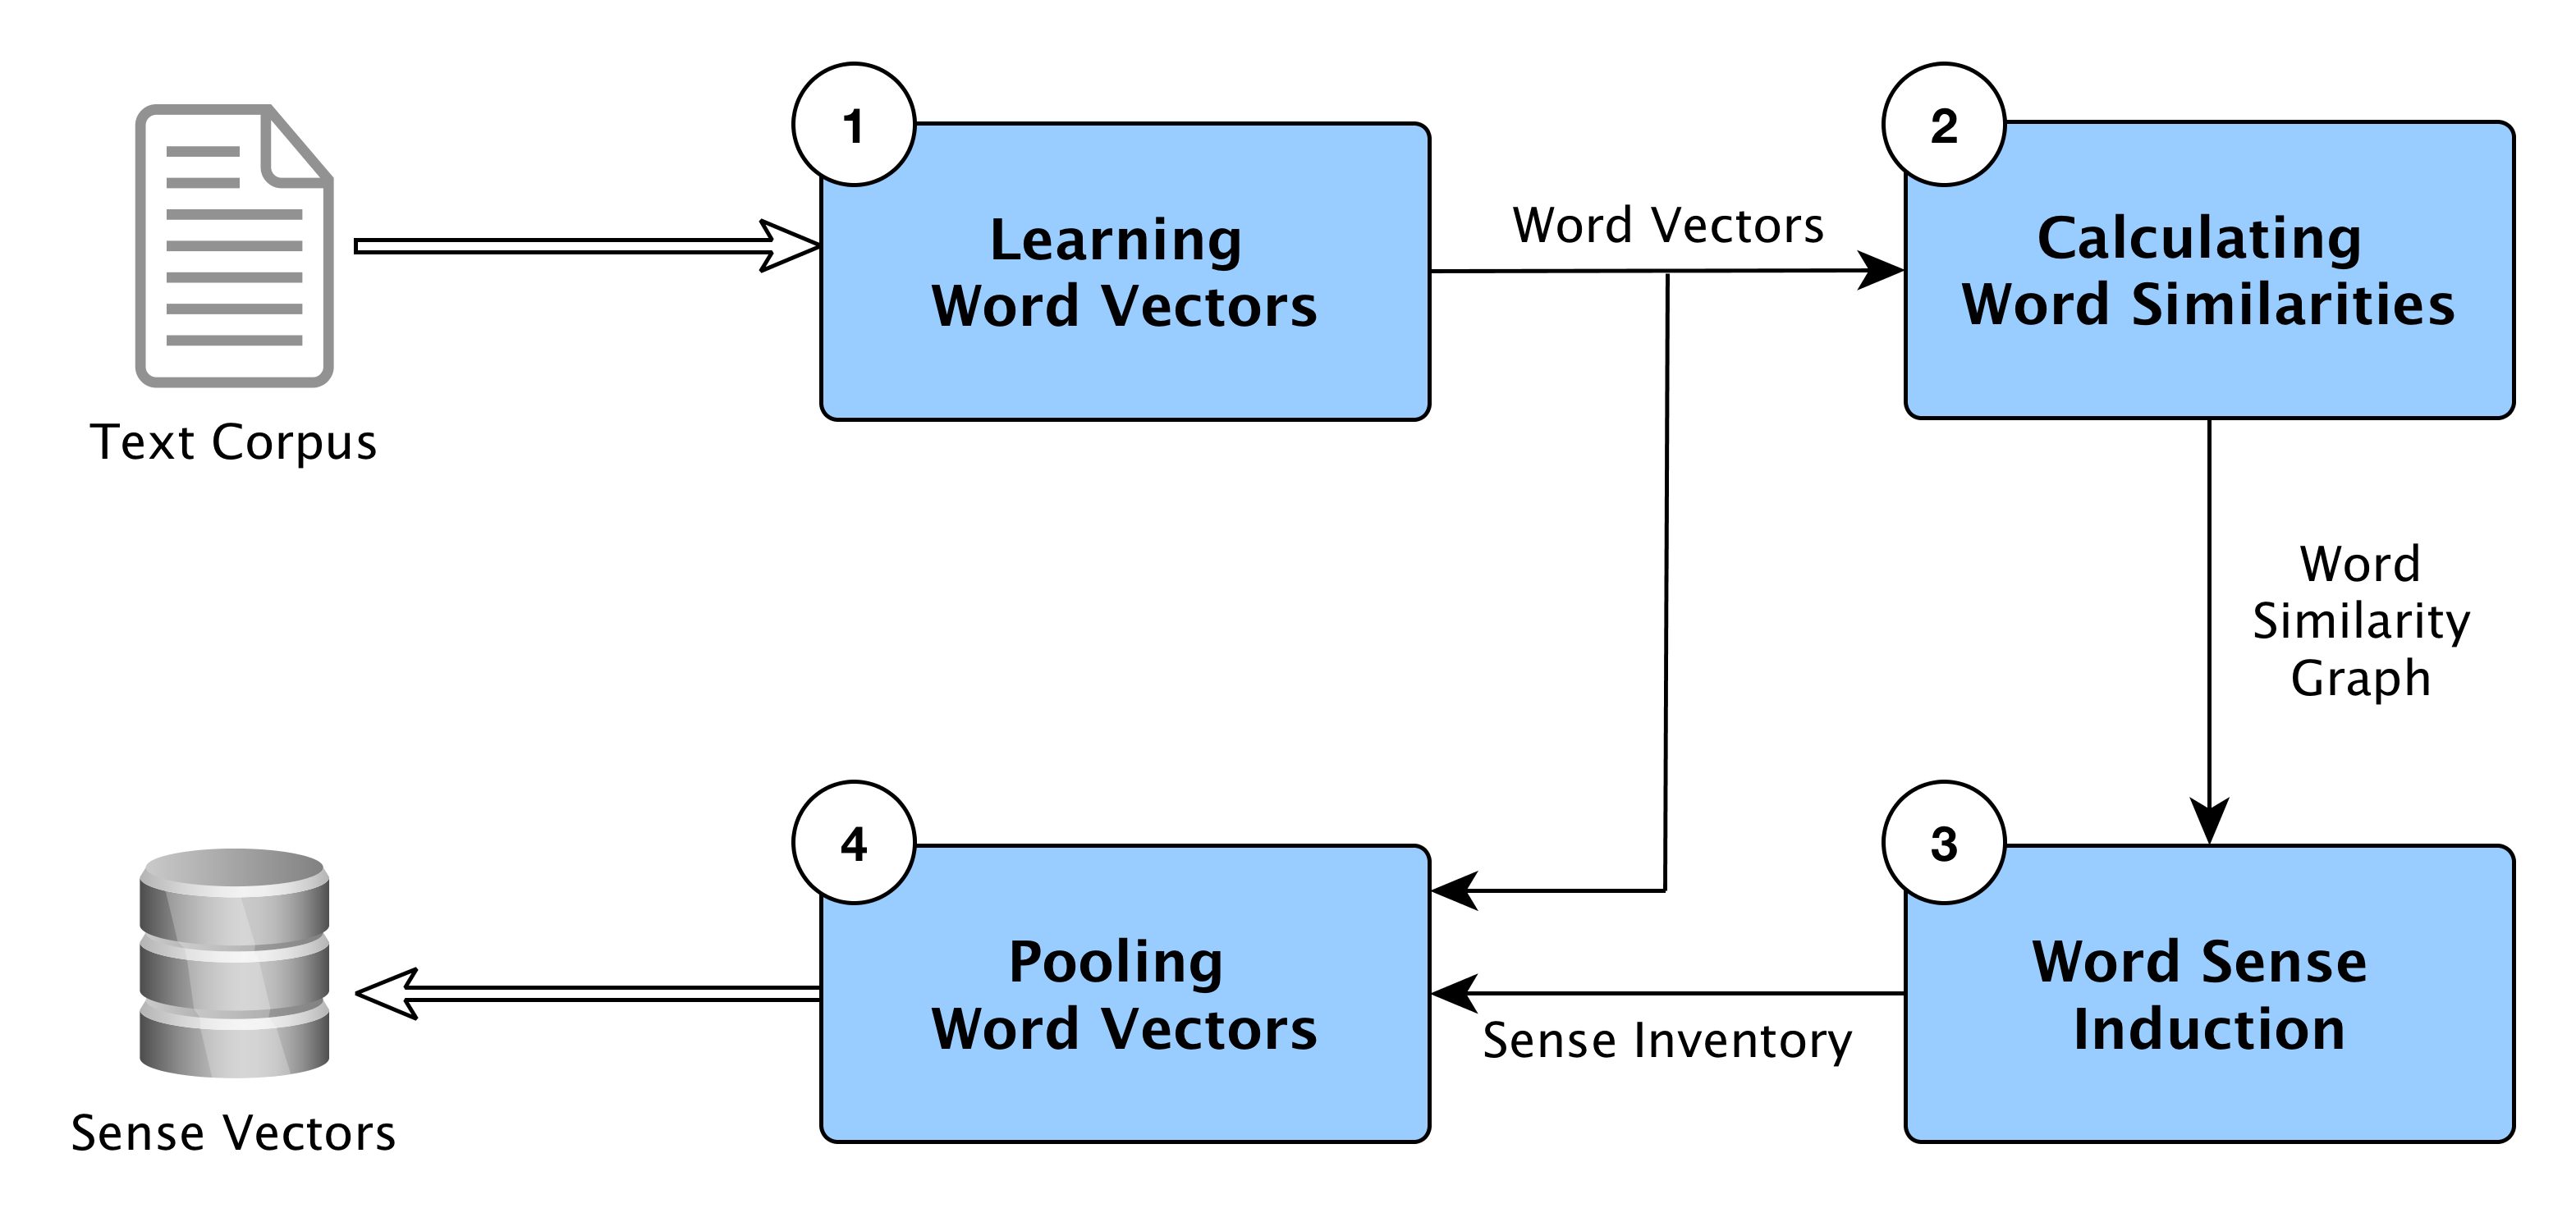
\includegraphics[width=\textwidth]{pipeline}
\end{frame}

\begin{frame}{Word Sense Induction: Ego-Network Clustering}

\centering
\begin{figure}
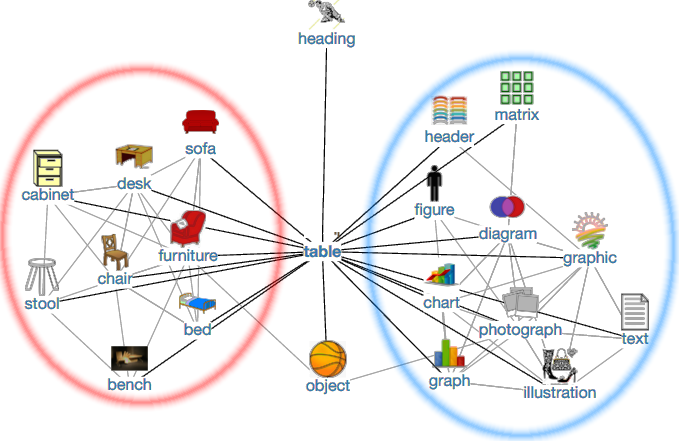
\includegraphics[width=0.65\textwidth]{table}
\end{figure}

\begin{itemize}
%\item Visualization of the ego-network of the word "table".\item The "furniture" and the "data" sense clusters of the word "table". 	
\item Graph clustering using the \textbf{Chinese Whispers algorithm} (Biemann, 2006).
\end{itemize}


\end{frame}


\begin{frame}{Neighbours of Word and Sense Vectors}


\begin{table}
\footnotesize
\centering
\begin{tabular}{l|l}
\toprule
\bf Vector & \bf \parbox{4cm}{Nearest Neighbours} \\ \midrule
 table & \parbox{6cm}{\alert{tray}, bottom, diagram, \alert{bucket}, brackets, stack, \alert{basket}, list, parenthesis, \alert{cup}, \alert{trays}, \alert{pile}, \alert{playfield}, bracket, \alert{pot}, drop-down, \alert{cue}, \alert{plate}} \\ \midrule
  table\#0 & \parbox{6cm}{leftmost\#0,  column\#1,  randomly\#0,  tableau\#1, top-left#0, indent\#1,  bracket\#3,  pointer\#0,  footer\#1, cursor\#1, diagram\#0, grid\#0} \\ \midrule
   table\#1 & \parbox{6cm}{ \alert{pile\#1,  stool\#1,  tray\#0,  basket\#0,  bowl\#1,  bucket\#0,  box\#0,  cage\#0,  saucer\#3,      mirror\#1,  birdcage\#0,  hole\#0,  pan\#1,  lid\#0} } \\ 
\bottomrule
\end{tabular}
\end{table}

\begin{itemize}
	\item Neighbours of the word ``table" and its senses produced by our method.
	\item The neighbours of the initial vector belong to \textbf{both senses}.
	\item The neighbours of the sense vectors are \textbf{sense-specific}.   
\end{itemize}

	
\end{frame}



\begin{frame}{Word Sense Disambiguation}
	\begin{block}{1. Context Extraction}
		\begin{itemize}
			\item use context words around the target word
		\end{itemize}
	\end{block}
	\vfill
	\begin{block}{2. Context Filtering}
		\begin{itemize}
			\item based on context word's relevance for disambiguation
		\end{itemize}
	\end{block}
	\vfill
	\begin{block}{3. Sense Choice}
		\begin{itemize}
			\item maximize similarity between context vector and sense vector
		\end{itemize}
	\end{block}
\end{frame}
	
\begin{frame}{Word Sense Disambiguation: Example\\ 
		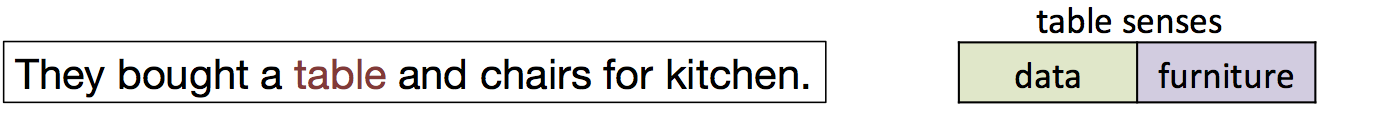
\includegraphics[width=0.85\textwidth]{wsd1}}
	\begin{center}
		\vspace{-0.3cm}
		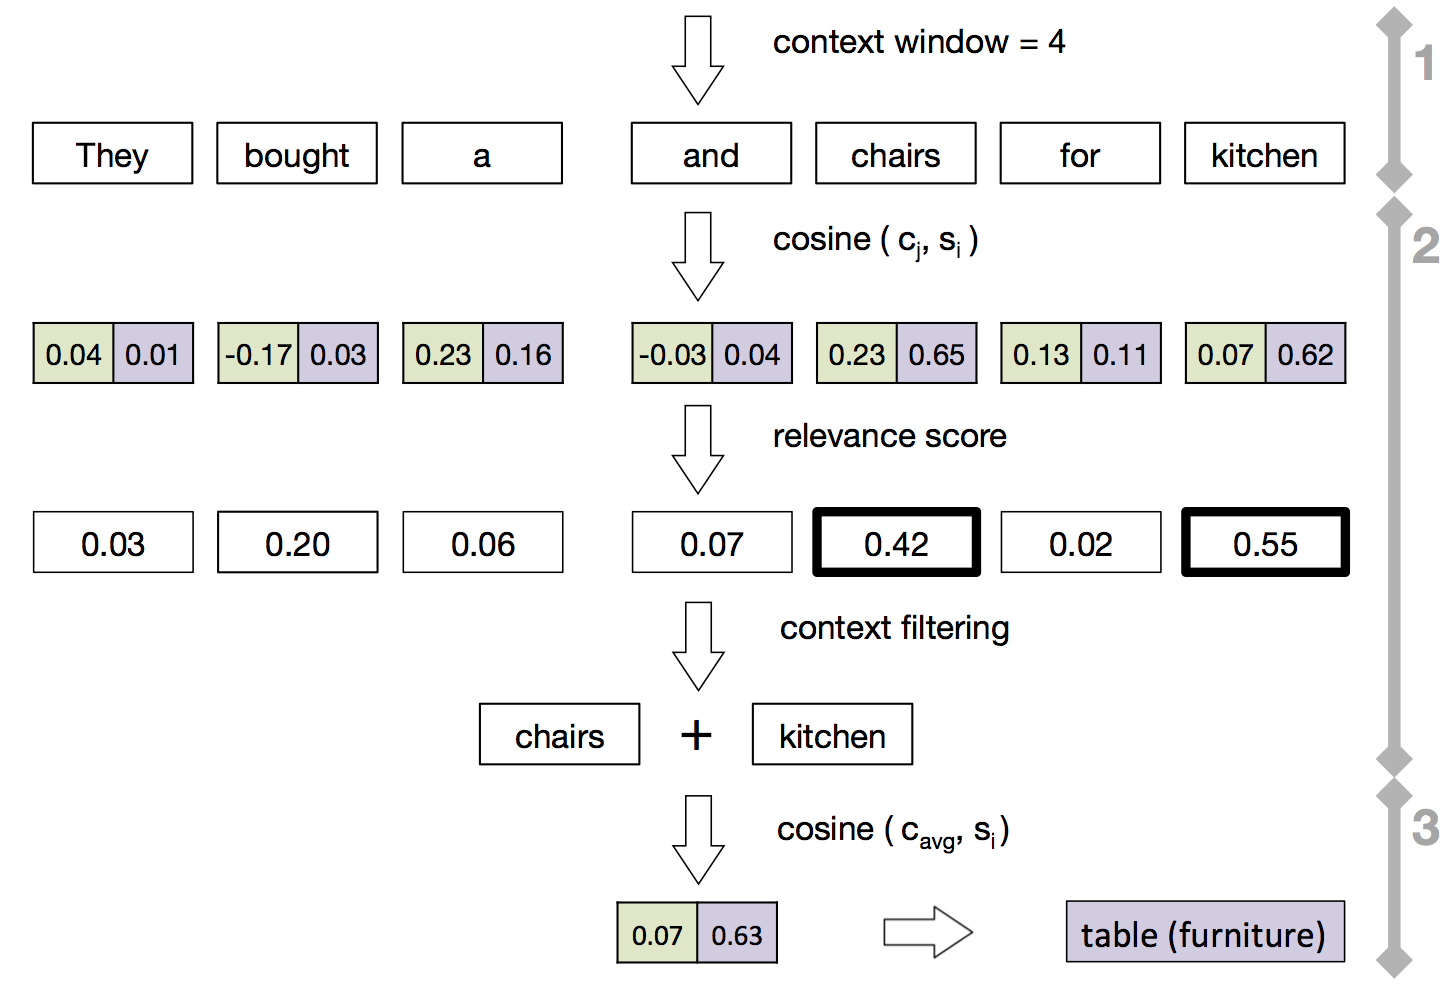
\includegraphics[width=0.75\textwidth]{wsd2}
	\end{center}
\end{frame}




\begin{frame}{Evaluation on SemEval 2013 Task 13 dataset: comparison to the state-of-the-art}
	\vspace{-0.4cm}
	\small
	\begin{center}
		\begin{tabular}{l|ccc|cc}
			\bf Model & \bf Jacc. & \bf Tau & \bf WNDCG & \bf F.NMI & \bf F.B-Cubed \\ 
			\midrule
			
			AI-KU (add1000) & 0.176 & 0.609 & 0.205 & 0.033 & 0.317 \\
			AI-KU & 0.176 & 0.619 & 0.393 & 0.066 & 0.382 \\
			AI-KU (remove5-add1000) & 0.228 & 0.654 & 0.330 & 0.040 & 0.463 \\
			Unimelb (5p) & 0.198 & 0.623 & 0.374 & 0.056 & 0.475 \\
			Unimelb (50k) & 0.198 & 0.633 & 0.384 & 0.060 & 0.494 \\
			UoS (\#WN senses) & 0.171 & 0.600 & 0.298 & 0.046 & 0.186 \\
			UoS (top-3) & 0.220 & 0.637 & 0.370 & 0.044 & 0.451 \\
			La Sapienza (1) & 0.131 & 0.544 & 0.332 & --  & -- \\
			La Sapienza (2) & 0.131 & 0.535 & 0.394 & -- & -- \\ \midrule
			AdaGram, $\alpha$ = 0.05, 100 dim & 0.274 & 0.644  & 0.318  & 0.058  & 0.470  \\ \midrule
			\alert{w2v}  & 0.197 & 0.615 & 0.291 & 0.011 & 0.615 \\
			%& \wv   -- weighted -- $$p=2$$ -- filter2 -- sw  & 0.197 & 0.614 & 0.291 & 0.012 & 0.615 \\
			\alert{w2v (nouns)} & 0.179 & 0.626 & 0.304 & 0.011 & 0.623 \\
			
			\alert{JBT} & 0.205 & 0.624 & 0.291 & 0.017 & 0.598\\
			\alert{JBT (nouns)} & 0.198 & 0.643 & 0.310 & 0.031 & 0.595\\
			\alert{TWSI (nouns)} & 0.215 & 0.651 & 0.318 & 0.030 & 0.573 \\ 
				
		\end{tabular}
	\end{center}
\end{frame}

%%%%%%%%%%%%%%%%%%%%%%%%%%%%%%%%%%%%%%%%%%%%%%%%%%%%%%%%%%%%%%%%%%%%%%%%%%%%%%%%%%%%%%%%%%%%%%%%%%%%%%%%%%%%%%%%%%%%%%%%%%%%%%%%%%%%%%%%%%%%
%\addtobeamertemplate{block begin}{\vspace*{-3pt}}{}
%\addtobeamertemplate{block end}{}{\vspace*{-3pt}}
\begin{frame}{Conclusion}
	\vfill
	\begin{itemize}
		\setlength{\itemsep}{1cm}
		\item Novel approach for learning \textbf{word sense embeddings}.
		\item Can use \textbf{existing word embeddings} as input.
		\item WSD performance \textbf{comparable to the state-of-the-art} systems.
		\item \alert{\textbf{Source code and pre-trained models:}} \url{https://github.com/tudarmstadt-lt/SenseGram}
		
	\end{itemize}
	\vfill
\end{frame}

%%%%%%%%%%%%%%%%%%%%%%%%%%%%%%%%%%%%%%%%%%%%%%%%%%%%%%%%%%%%%%%%%%%%%%%%%%%%%%%%%%%%%%%%%%%%%%%%%%%%%%%%%%%%%%%%%%%%%%%%%%%%%%%%%%%%%%%%%%%%

\begin{frame}{}
	\vfill
	\begin{center}
		\alert{\textbf{\LARGE Thank you and welcome to our poster!}}
	\end{center}
	\vfill
\end{frame}


\begin{frame}{Evaluation based on the TWSI dataset: a large-scale dataset for development}
	\begin{center}
			\vspace{1.2cm}

		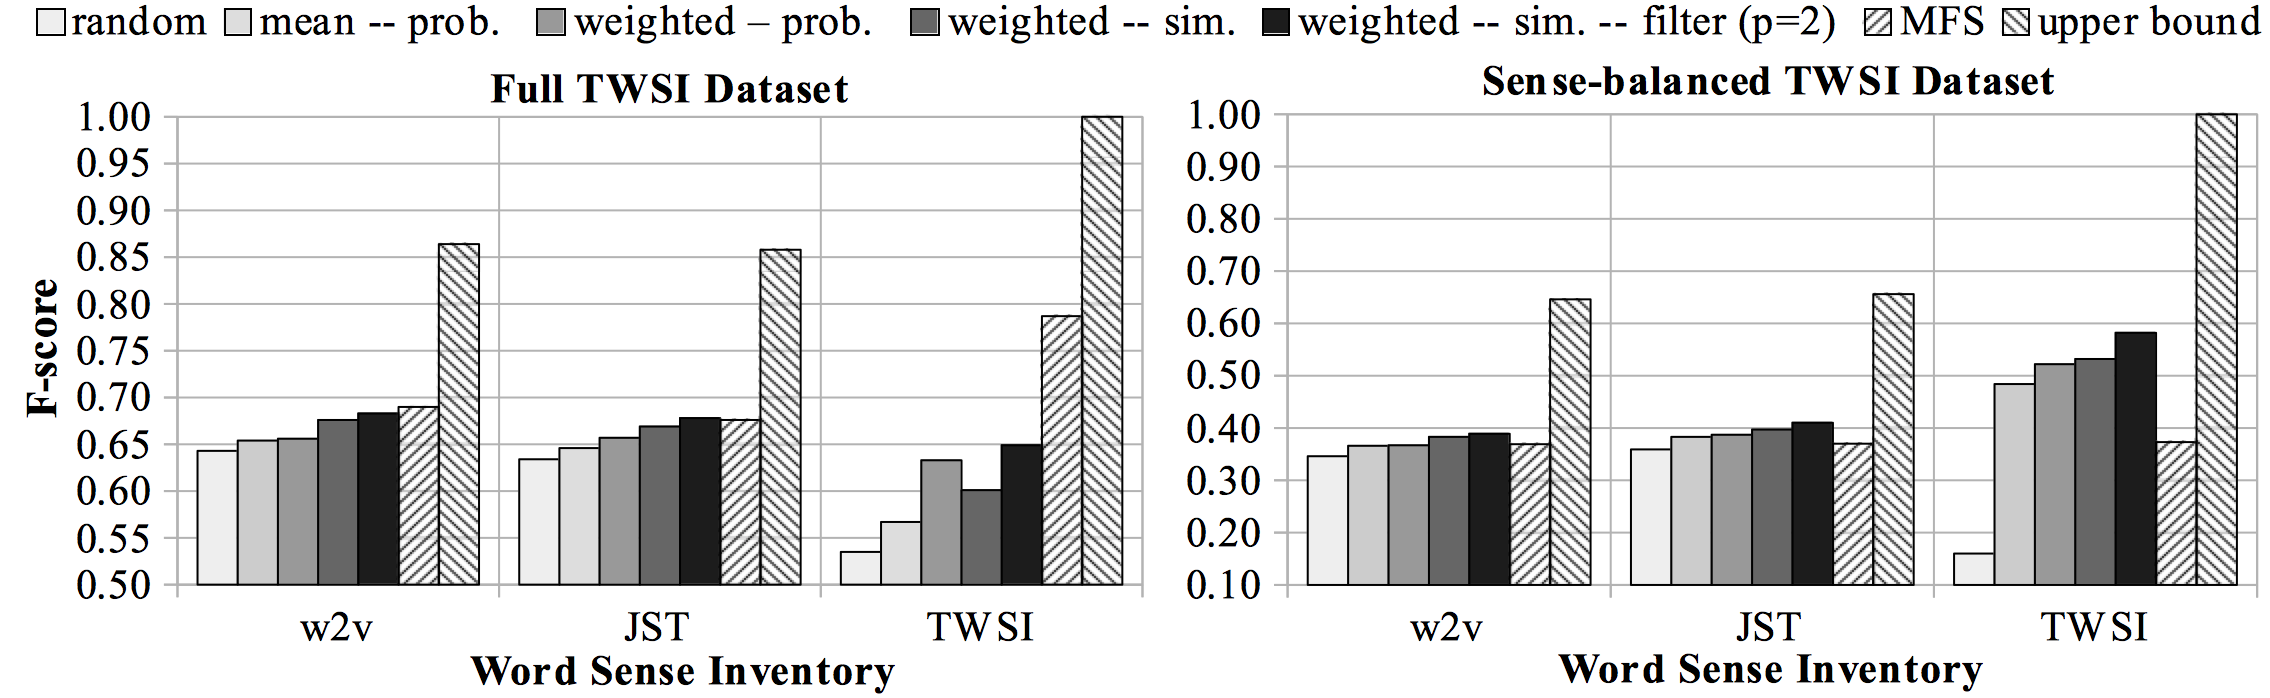
\includegraphics[width=1.0\textwidth]{results-plot}
	\end{center}
\end{frame}


\end{document}
